%; whizzy chapter -dvi
% -initex iniptex -latex platex -format platex -bibtex jbibtex -fmt fmt
% 以上 whizzytex を使用する場合の設定。

%     Tokyo Debian Meeting resources
%     Copyright (C) 2012 Junichi Uekawa
%     Copyright (C) 2011 Nobuhiro Iwamatsu

%     This program is free software; you can redistribute it and/or modify
%     it under the terms of the GNU General Public License as published by
%     the Free Software Foundation; either version 2 of the License, or
%     (at your option) any later version.

%     This program is distributed in the hope that it will be useful,
%     but WITHOUT ANY WARRANTY; without even the implied warranty of
%     MERCHANTABILITY or FITNESS FOR A PARTICULAR PURPOSE.  See the
%     GNU General Public License for more details.

%     You should have received a copy of the GNU General Public License
%     along with this program; if not, write to the Free Software
%     Foundation, Inc., 51 Franklin St, Fifth Floor, Boston, MA  02110-1301 USA

%  preview (shell-command (concat "evince " (replace-regexp-in-string "tex$" "pdf"(buffer-file-name)) "&"))
% 画像ファイルを処理するためにはebbを利用してboundingboxを作成。
%(shell-command "cd image201307; ebb *.jpg")

%%ここからヘッダ開始。

\documentclass[mingoth,a4paper]{jsarticle}
\usepackage{monthlyreport}

% 日付を定義する、毎月変わります。
\newcommand{\debmtgyear}{2013}
\newcommand{\debmtgmonth}{7}
\newcommand{\debmtgdate}{20}
% started from zero:
% (let ((year 2013) (month 7)) (+ (* (- year 2005) 12) month -1))
\newcommand{\debmtgnumber}{102}

\begin{document}

\begin{titlepage}
\thispagestyle{empty}
% タイトルページ:編集必要な部分は最初のマクロに飛ばすこと

\vspace*{-2cm}
第\debmtgnumber{}回 東京エリア Debian 勉強会資料\\
\hspace*{-2cm}

\includegraphics{image2012-natsu/dotdeb.pdf}\\
\hfill{}\debmtgyear{}年\debmtgmonth{}月\debmtgdate{}日

% ここはアップデートすること
% 全角文字にしないとフォントのサイズが合わないので注意
\rotatebox{10}{\fontsize{32}{32} {\gt 特集1: Debian armmp / Raspberry Pi}}

\rotatebox{10}{\fontsize{32}{32} {\gt 特集2: 月刊Debhelper: dh\_strip }}

\vspace*{-2cm}
\hfill{}
\includegraphics[height=6cm]{image200502/openlogo-nd.eps}
\end{titlepage}

\dancersection{Introduction}{上川 純一}

\begin{multicols}{2}
 

 今月のDebian勉強会へようこそ。これからDebianの世界にあしを踏み入れると
 いう方も、すでにどっぷりとつかっているという方も、月に一回Debianについ
 て語りませんか?

 Debian勉強会の目的は下記です。

 \begin{itemize}
 \item \underline{Debian Developer} (開発者)の育成。
 \item 日本語での「\underline{開発に関する情報}」を整理してまとめ、アップデートする。
 \item \underline{場}の提供。
 \begin{itemize}
  \item 普段ばらばらな場所にいる人々が face-to-face で出会える場を提供
	する。
  \item Debian のためになることを語る場を提供する。
  \item Debianについて語る場を提供する。
 \end{itemize}
 \end{itemize}		

 Debianの勉強会ということで究極的には参加者全員がDebian Packageをがりがり
 と作るスーパーハッカーになった姿を妄想しています。情報の共有・活用を通し
 て Debianの今後の能動的な展開への土台として、「場」としての空間を提供す
 るのが目的です。

\end{multicols}

\newpage

\begin{minipage}[b]{0.2\hsize}
 \definecolor{titleback}{gray}{0.9}
 \colorbox{titleback}{\rotatebox{90}{\fontsize{80}{80} {\gt デビアン勉強会} }}
\end{minipage}
\begin{minipage}[b]{0.8\hsize}
\hrule
\vspace{2mm}
\hrule
\begin{multicols}{2}
\tableofcontents
\end{multicols}
\vspace{2mm}
\hrule
\end{minipage}

\dancersection{事前課題}{上川 純一}

今回の事前課題は以下です:
\begin{enumerate}
 \item お使いのマシンにARMはありますか?もしあるのでしたら、どのように使っているか教えてください。
 \item Debian のARM に期待していること、お願いしたいことがあれば教えてください。
\end{enumerate}
この課題に対して提出いただいた内容は以下です。
\begin{multicols}{2}
{\small

\begin{prework}{ koedoyoshida }

\begin{enumerate}
\item お使いのマシンにARMはありますか?もしあるのでしたら、どのように使っ
ているか教えてください。\\
Raspberry Piを使ってます。
とりあえずリモートアクセス用がメインですが、
I2Cとかを使って外部IOをやってみたいと思っています。
\item  Debian のARM に期待していること、お願いしたいことがあれば教えてくだ
さい。\\
省電力な環境を生かしてReadOnlyboot(でも定期的にセキュリティupdateはし
たい)で放置できる環境とかが作れるとよいですね。
\end{enumerate}

\end{prework}

\begin{prework}{ 吉野 }
\begin{enumerate}
\item  地図マシンです
\item なし 
\end{enumerate}
\end{prework}

\begin{prework}{ dictoss}
\begin{enumerate}
\item  CuBoxを持っている。eSATA端子があるのでファイルサーバのバックアップ
をするマシンとして使おうとしたが、USBポートから電源供給量が不足のため、
HDDが動かず使えていない。そのため単なるarmelバイナリのお試しマシンになっ
ている。

\item  新Nexus7でDebianが動いてほしい。
\end{enumerate}
\end{prework}

\begin{prework}{ mtoshi.g }
\begin{enumerate}
\item  お使いのマシンにARMはありますか?\\
ないっす

\item  Debian のARM に期待していること、お願いしたいことがあれば教えてくだ
さい。\\
今のところないっす
\end{enumerate}
\end{prework}

\begin{prework}{ 野島 貴英 }
\begin{enumerate}
\item  昔売っていたB\&NのNookColorをARM機材実験ボードとして未だに使ってます。
この電子書籍端末は2012/4の東京エリアdebian勉強会,2012/6の大統一debian
勉強会で喋ったとおり、特定ブートフォーマットのSDカードを用意してSDカー
ドスロットへ入れちゃうと、うっかりそのままブートしちゃうという隠れ(?)
機能が大変便利です。おまけに連続8回起動失敗するとリカバリーが始まると
いう非文鎮化機能まで搭載しています。そのままでもpdfリーダ、ポータブル
mp4ビデオ/mp3鑑賞機材として、また、debian ARMのnativeブートの可能性を
秘めたhack機材としても楽しくお使いいただけます。
\item  NookColor用のdebianネイティブブートが可能なイメージ(というかインス
  トーラ)が欲しいといってみるテスト。
\end{enumerate}
\end{prework}

\begin{prework}{ 岩松 信洋 }
\begin{enumerate}
\item  お使いのマシンにARMはありますか?もしあるのでしたら、どのように使っ
ているか教えてください。\\
たくさんある。開発用とかビルドマシンとして使っています。
Raspberry Pi は家のゲートウェイマシンとして動いています。
\item  Debian のARM に期待していること、お願いしたいことがあれば教えてくだ
さい。\\
マルチメディア系が弱いので整備して欲しい。
\end{enumerate}

\end{prework}

\begin{prework}{ 上川純一 }
なし
\end{prework}

\begin{prework}{ まえだこうへい }
\begin{enumerate}
\item  Armadillo Jで自宅内のDHCPサーバとして使っています(not Debian)。
OpenBlockS AX3を、昨年夏ごろにカッとなって作ったioriというツール(最近
話題のdockerみたいなの)の開発環境として使っています。
\item  今は特にないですが、今後ARMサーバの製品版が出てきた時にd-iでインス
トールできることでしょうか。
\end{enumerate}
\end{prework}

}
\end{multicols}

\dancersection{Debian Trivia Quiz}{上川純一}

ところで、みなさん Debian 関連の話題においついていますか?Debian関連の話
題はメーリングリストをよんでいると追跡できます。ただよんでいるだけではは
りあいがないので、理解度のテストをします。特に一人だけでは意味がわからな
いところもあるかも知れません。みんなで一緒に読んでみましょう。

今回の出題範囲は\url{debian-devel-announce@lists.debian.org} や \url{debian-devel@lists.debian.org}に投稿された
内容とDebian Project Newsからです。

\begin{multicols}{2}
%; whizzy-master ../debianmeetingresume201211.tex
% 以上の設定をしているため、このファイルで M-x whizzytex すると、whizzytexが利用できます。
%

\santaku
{Stefano Zacchiroli さんが新しく作成したサービスは?}
{chiebukuro.debian.net}
{2ch.debian.net}
{sources.debian.net}
{C}
{Stefano Zacchiroli さんが、Debian パッケージで提供されているソースコードすべてを閲覧・検索出来るsources.debian.netを作った}

\santaku
{新しく FTP master チームに入った人は?}
{Gergely Nagy} % 2012 DPL立候補者 % dh-exec 開発者
{Kouhei Maeda}
{Joerg Jaspert}
{A}
{Paul Tagliamonte,Scott Kitterman,Luke Faraone, Gergely Nagy が加入}

\santaku
{Debian GNU/Hurd がリリースされましたが、バージョンはいくつでしょう。}
{2013}
{3.141592}
{7.0}
{A}
{}


\end{multicols}

\dancersection{最近のDebian関連のミーティング報告}{上川純一}
\subsection{東京エリアDebian勉強会100回目報告}

% (query-replace-regexp "<.*?>" "")
% (query-replace-regexp "^[	 ]\+" "")

%-------------------------------------------------------------------------------
\dancersection{Debian linux kernel / armmp フレーバ}{岩松 信洋}
%-------------------------------------------------------------------------------
\index{armmp}

\subsection{はじめに}
Debian linux kernel の3.9 から armhf アーキテクチャに armmp (ARM Multi Platform) 
フレーバが入りました。
本稿では armmp の仕組みと対応方法について説明します。

\subsection{arm multi platformとその仕組み}

Linux kernel バージョン3.8 ぐらいからarm multi platform(以下、ARMMP) サポートが入りました。
これは一つの linux kernel バイナリで複数のARM Soc、ターゲットボードをサポートする仕組みです。
今のところ、mvebu (Marvell SoCs)を筆頭に Versatile Express、OMAP などがサポートされて
います。バージョン3.11 ではほとんどのARM SoCがサポートされる予定になっています。

複数SoCやターゲットボードへの対応方法ですが、これはカーネル起動時にDevice Tree (以下、DT)と
呼ばれるハードウェア情報を渡すことによって、カーネルを各デバイス向けに初期化し動作するように
なります。

\subsubsection{ARMMP カーネルの起動方法}
通常Linuxカーネルを起動する場合、zImage だけで起動しますが、ARMMPや最近のARM向けカーネルはDTが
必要になっています。
DTを絡めたカーネル起動方法は3つほどあります。起動方法別にLinux上での操作(linux\$がlinux上での操作)
とU-Boot
\footnote{U-Boot は ARM 組込機器でよく利用されるブートローダ}
上での操作
(u-boot\$はU-boot上での操作)
を以下に紹介します。

\begin{enumerate}
\item zImageにdtb (DT blob。DTのバイナリ)を付加する。そしてそのzImageで起動する。\\
まずカーネルのCONFIG\_ARM\_APPENDED\_DTBが必要です。有効になっていない場合は有効にしましょう。
そしてビルドされたzImageとdtbを結合します。
\begin{commandline}
linux$ cat arch/arm/boot/zImage arch/arm/boot/dts/armada-xp-openblocks-ax3-4.dtb  > arch/arm/boot/zImage+dtb 
\end{commandline}
%$
上で作成した zImage+dtb をターゲット機器上にコピーします。以下の例は tftp を使って0x2000000にコピーしています。
0x2000000 はターゲットによって異なるので環境に合わせて変更してください。
そして\texttt{go} コマンドに ロードしたアドレスを指定して実行し、カーネルを起動させています。

\begin{commandline}
u-boot$ tftpboot 2000000 zImage+dtb
u-boot$ go 2000000 
\end{commandline}
%$

\item 1. で作成したzImage を uImage に変換して起動する。

以下は 結合したイメージを uImage 形式に変換しています。
最初の\texttt{make uImage}では zImage を uImage に変換していますが、その後zImageとdtbを結合(zImage+dtb)し、
\texttt{arch/arm/boot/.uImage.cmd}を使って結合したイメージをuImage(uImage+dtb)に変換しています。
\footnote{後述するmkimageを直接呼んでもよい}
\begin{commandline}
linux$ make uImage
linux$ cat arch/arm/boot/zImage arch/arm/boot/dts/armada-xp-openblocks-ax3-4.dtb  > arch/arm/boot/zImage+dtb 
linux$ `cut -f 3- -d ' ' < arch/arm/boot/.uImage.cmd | sed -e 's/zImage/zImage+dtb/g' -e 's/uImage/uImage+dtb/g'`
\end{commandline}
%$

起動に利用するフォーマットがuImage形式の場合、\texttt{go}コマンドではなく \texttt{bootm}コマンドのを使います。
\begin{commandline}
u-boot$ tftpboot 2000000 uImage+dtb
u-boot$ bootm
\end{commandline}
%$
これらの方法は ARMMP ではない SoC単体でDTを使う場合のみ有効です。
カーネルがロードされるアドレスなどはSoCやボード毎に異なるのですが、SoC単体では
カーネルのコンフィグ情報としてこれらを持っているので上記の説明で uImage が作成できます。
しかしARMMPの場合はSoC毎にこれらの値が異なるのでターゲットSoC毎にこれらの値を変更する
必要があります。ARMMP で実行すると以下のようなエラーになるでしょう。

\begin{commandline}
linux$  `cut -f 3- -d ' ' < arch/arm/boot/.uImage.cmd | sed -e 's/zImage/zImage+dtb/g' -e 's/uImage/uImage+dtb/g'`
  CHK     include/generated/uapi/linux/version.h
  CHK     include/generated/utsrelease.h
make[1]: `include/generated/mach-types.h' is up to date.
  CALL    scripts/checksyscalls.sh
  CHK     include/generated/compile.h
  Kernel: arch/arm/boot/Image is ready
  Kernel: arch/arm/boot/zImage is ready
multiple (or no) load addresses: 
This is incompatible with uImages
Specify LOADADDR on the commandline to build an uImage
make[1]: *** [arch/arm/boot/uImage] Error 1
make: *** [uImage] Error 2
\end{commandline}

ロードアドレスなどの情報はmkimage
\footnote{U-Boot 用のイメージを作成するツール。}
で指定できます。
\footnote{arch/arm/boot/.uImage.cmd 内では mkimage を呼んでいる}

\texttt{-a} でロードアドレス、\texttt{-e}でエントリポイントアドレスを指定します。
\begin{commandline}
linux$ cat zImage foo.dtb > zImage+dtb 
linux$ mkimage -A arm -O linux -T kernel -C none -a 0x2000000 -e 0x2000040 -n 'Linux-marvell' -d arch/arm/boot/zImage+dtb arch/arm/boot/uImage+dtb
\end{commandline}
\footnote{カーネル開発者は./scripts/mkuboot.sh を使う事が多いかも。}
%$

\item uImage と dtb blob 別に読み込んで起動する。

ARMMP は 一つのバイナリで複数のARM SoC、ボードをサポートすることが目的なので、上記の方法ではサポートできません。
よって、uImage と dtb blob を分けて起動させるのが理想です。
U-Boot の場合は カーネルを起動するコマンド\texttt{bootm} を使います。

\begin{commandline}
linux$ mkimage -A arm -O linux -T kernel -C none -a 0x2000000 -e 0x2000040 -n 'Linux-marvell' -d arch/arm/boot/zImage arch/arm/boot/uImage
\end{commandline}
%$

\begin{commandline}
u-boot$ tftpboot 2000000 uImage
u-boot$ tftpboot 3000000 dtb
u-boot$ bootm 2000000 - 3000000
\end{commandline}
%$
%$

bootmコマンドの 第1引数はuImage がロードされているアドレス、第2引数は uInitrd(initrd イメージのuImage)がロードされている
アドレス、第3引数には dtb がロードされているアドレスを指定します。\texttt{-}は 指定なしを意味します。

ちなみにdtb の格納されてるアドレスはブートローダによってカーネル起動時の r2 レジスタに設定され、カーネルが指定されているアドレスから
データを読み込み起動する用になっています。これは Linux カーネルの Documentation/arm/Bootingに書かれています。

\end{enumerate}

\subsubsection{カーネルモジュールの対応}

カーネルモジュールもDTによって設定できます。
必要なカーネルドライバを組み込みにしてカーネルを起動させるのもよいのですが、ARMMPの場合
カーネルが肥大化しますので、SoCのコア部分は最低限の機能は組み込みに設定し、各デバイス用
ドライバはモジュールにしてinitrd などからロードするようにするのがよいでしょう。
Debianの場合はサポートボード毎にzImage を用意せず、上記の方法で対応しています。

\subsection{Debianでのサポート}

Debianのarmhf アーキテクチャの armmp フレーバ は上記で説明した機能を持ったカーネルをサポートするためのものです。
今回 Plat'Homeさん\footnote{\url{http://www.plathome.co.jp/}}
の Openblocks AX3 をDebianでサポートするために実装しました。
AX3 は \texttt{mvebu} という Marvell製 SoC をまとめている SoC アーキテクチャとしてサポートされているのですが、
これはARMMP サポートのみで実装されているので、Debian側でもARMMPサポートする必要がありました。
また、他の今後ARMカーネルはARMMPに移行することが決定していたので、誰かやる必要があったというのも理由の一つです。

\subsection{Debianでのカーネル提供と利用方法}
Debian はカーネルイメージを uImage で提供していません。
uImage で提供した場合、カーネルがロードされるアドレスが固定値になってしまうので、複数のデバイスをサポート
できません。Debianでは カーネルをzImage(vmlinuz) として提供しています。

しかしこのままでは U-Boot を使ったデバイスなどで使う場合に手間がかかるので、
Debian では flash-kernel\footnote{\url{http://packages.qa.debian.org/f/flash-kernel.html}} 
パッケージでサポートしています。

flash-kernel は設定されたデータをもとにカーネルやinitrdをU-Bootなどで扱える形式に変換し、
フラッシュメモリに書き込む機能等を提供します。

データの形式は以下のようになります。このデータは\texttt{/usr/share/flash-kernel/db/all.db}に
記述されます。

\begin{commandline}
Machine: Marvell Armada 370/XP (Device Tree)
Kernel-Flavors: armmp
DTB-Id: armada-xp-openblocks-ax3-4.dtb
DTB-Append: yes 
U-Boot-Kernel-Address: 0x2000000
U-Boot-Initrd-Address: 0x0
Boot-Device: /dev/sda1
Boot-Kernel-Path: /boot/uImage
Boot-Initrd-Path: /boot/uInitrd
Required-Packages: u-boot-tools
Bootloader-Sets-root: no
\end{commandline}

flash-kernel を実行すると設定されているデータと起動しているカーネル情報
(/proc/cpuinfo、または/proc/device-tree/model)を元にカーネルとinittd を
変換し、インストールします。
\begin{commandline}
$ cat /proc/cpuinfo | tail -3
Hardware        : Marvell Armada 370/XP (Device Tree)
Revision        : 0000
Serial          : 0000000000000000

$ flash-kernel 
flash-kernel: installing version 3.10-1-armmp
Generating kernel u-boot image... done.
Installing new uImage.
Generating initramfs u-boot image... done.
Installing new uInitrd.
Installing new dtb.

$ ls /boot
System.map-3.10-1-armmp  initrd.img-3.10-1-armmp  uInitrd
config-3.10-1-armmp      uImage                   vmlinuz-3.10-1-armmp
\end{commandline}
%$ 

flash-kernel によって作成されたイメージを使った起動方法はボード毎に異なります。
OpenBlocks AX3の場合は以下の方法で起動できるはずです。

\begin{commandline}
$ ide reset
$ ext2load ide 0 2000000 /boot/uImage
$ ext2load ide 0 3000000 /boot/uInitrd
$ bootm 2000000 3000000
\end{commandline}


\subsection{終わりに}

ARMMP の仕組みと、Debianの対応方法について説明しました。
flash-kernel のデータはぷらっとホームさんと相談して入れようと思っているのでまだコミットされていません。
数日後にはパッチがBTSに上がるでしょう。OpenBlocks A6 もサポートします。
また、エントリーポイントを設定する項目とDTの model を指定する項目がないのでこれも対応する必要があります。
パッチはつくってあるので後日BTSします。
あと、残作業としてはカーネル 3.10 では mvebu が動作しない(他でも同じかも)のでパッチを当てる必要があります
(コミット: \texttt{faefd550c45d8d314e8f260f21565320355c947f})。これもBTSします。
ということでまだまだやることはたくさんあります。

%-------------------------------------------------------------------------------
\dancersection{月刊Debhelper dh\_strip}{野島 貴英}
%-------------------------------------------------------------------------------
\index{dh\_strip}

\subsection{今月のコマンド}

 今月はdh\_stripを取り上げます。紙面の都合でdh\_stripの1コマンドの
紹介に今回はとどめておきます。

\subsection{dh\_strip}

 dh\_stripコマンドは、 ``debian/tmp/'' 等のビルドディレクトリ以下を再帰的に
探し回り、ビルドしたばかりの実行ファイルのバイナリ、共有ライブラリのバイナリ、静的ライブラリのバイナリを見付けると、片っ端からバイナリに含まれているデバッグシンボルを取り除いてくれます。

 また、別途コマンドラインオプションを指定すると、取り除いたデバッグシンボルを別ファイルに取り置きます。このため、dh\_stripコマンドは*-dbgパッケージ作成の時に重要な役割を持ちます。

\subsubsection{すでに発表済みの件}

 実は、dh\_stripの*-dbgパッケージを作成する為の動作については、大統一Debian 2012のセッションである「debug.debian.net」\cite{debug-debian-net}のプレゼン資料に詳しいので、こちらを参照してください。

 また、*-dbgパッケージを使って実際にデバッグをしてみる件については、大統一Debian 2013のセッションである「gdb+python拡張を使ったデバッグ手法」\cite{gdb-python-debug2}に紹介していますので、こちらも参照ください。

 ここでは、これらの発表で扱わなかった件を重点的に記載します。

\subsubsection{debug/*.so,lib*\_g.aファイルの扱い}

 dh\_stripコマンドは、元々デバッグ用途として用意されているdebug/*.soファイルや、
lib*\_g.aファイルについては、何も処理を行いません。

\subsubsection{コマンドラインオプションと動作}

 dh\_stripコマンドは表\ref{tab:dh-strip-opt}のコマンドラインオプションを解釈します。

\begin{table}[ht]
\begin{center}
\small
\begin{tabular}{|p{8em}|p{35em}|}
\hline
オプション名&動作 \\ \hline \hline
man debhelper記載のオプション & こちらは全debhelperに共通のオプションです。動作はman debhelperに記載されていたり、以前の月刊debhelperで説明されているとおりとなりますので、ここでは割愛します。 \\ \hline
-Xitem, --exclude=item & itemで指定されるファイル名を持つバイナリを処理の対象から外します。複数のファイルを指定したい場合は、繰り返し指定すると指定できます。例: dh\_strip -Xfile1 -Xfile2 \\ \hline
--dbg-package=package & *-dbgパッケージを作る際に、デバッグシンボルを格納するパッケージ名を指定する為に利用します。通常、*-dbgパッケージを作る場合は、こちらのオプションを利用する事となります。なお、ソースパッケージにあるdebian/compatで指定されるCOMPATIBILITY LEVELで振る舞いが異なります(後述)。\\ \hline
-k & 分離したデバッグシンボルをバイナリパッケージに含める場合にこちらのオプションを利用します。この場合、出来上がったパッケージにはバイナリの他に、分離したデバッグシンボルも/usr/lib/debug/以下に含まれる形で収録されます。--dbg-packageが同時に指定されると、--dbg-packageの指定の方が優先されます。\\ \hline
\end{tabular}
\caption{dh\_stripコマンドラインオプション}
\label{tab:dh-strip-opt}
\end{center}
\end{table}

\subsubsection{COMPATIBILITY LEVELでの動作の違い}

 dh\_stripはソースパッケージに含まれるdebian/compatで指定される
COMPATIBILITY LEVELにより、振る舞いが変わります。

 --dbg-packageオプション指定時の振る舞いの違いは表\ref{tab:dh-strip-comp-level}に、
また、-k/--dbg-packageオプション指定時に生成されるデバッグシンボルファイルの違いについて表\ref{tab:debugsym-file-difference-comp-level}に、記載します。

\begin{table}[ht]
\begin{center}
\small
\begin{tabular}{|p{8em}|p{35em}|}
\hline
COMPATIBILITY LEVEL &--dbg-package指定時の動作 \\ \hline \hline
4以下 & ``dh\_strip --dbg-package=xxxx --dbg-package=yyyy''のように--dbg-packageを複数指定する事が出来ます。ここで、こちらで指定した名前(xxxxや、yyyy)に合致するパッケージを処理する際、''パッケージ名-dbg''というパッケージ名を*-dbgパッケージのパッケージ名として自動的に利用します。また、ソースパッケージに含まれるdebian/controlには、これら*-dbgパッケージの為の記述は不要となります。\\ \hline
5以上 & --dbg-packageは1つ指定するのが原則となります。もし複数指定した場合は、最初に指定された内容のみ利用されます。また、--dbg-package=xxxxxとすると、デバッグシンボルを格納するパッケージ名として、xxxxxがそのまま使われます。例えば、libfooパッケージと、fooパッケージを構築し、これらパッケージに含まれているバイナリのデバッグシンボルをfoo-dbgパッケージに全部入れるには、--dbg-package=foo-dbgと指定します。また、
ソースパッケージに含まれるdebian/controlには、生成予定の*-dbgパッケージの為の記述は必須となり、万一記載されていない場合はエラーとして扱われ、この場合はdh\_stripはエラーを表示して終了します。\\ \hline
\end{tabular}
\caption{COMPATIBILITY LEVELと--dbg-packageオプションの振る舞いの違い}
\label{tab:dh-strip-comp-level}
\end{center}
\end{table}

\begin{table}[ht]
\begin{center}
\small
\begin{tabular}{|p{8em}|p{35em}|}
\hline
COMPATIBILITY LEVEL &-k/--dbg-package指定時のデバッグシンボルファイルの違い \\ \hline \hline
8以下 & ``/usr/lib/debug/+バイナリのインストール先パス/+バイナリファイル名''に格納されるようにデバッグシンボルファイルが生成されます。また、デバッグに関する情報はコンパイラが生成したままの形で保存されるため、デバッグシンボルファイルのサイズは大きくなりがちです。\\ \hline
9以上 & バイナリがBuildID\cite{gdb-python-debug2}を含んでいる場合は、``/usr/lib/debug/.build-id/BuildIDの上位2桁/+BuildIDの残りの桁+.debug''に格納されるようにデバッグシンボルファイルが生成されます。BuildIDを含んでいなければCOMPATIBILITY LEVEL 8以下と同様のファイル名となります。また、BuildIDの有無にかかわらず、デバッグに関する情報はzlibにより圧縮されて格納されます。そのため、デバッグシンボルファイルのサイズはできるだけ小さくなるようになっています。\\ \hline
\end{tabular}
\caption{COMPATIBILITY LEVELと-k/--dbg-packageオプションの振る舞いの違い}
\label{tab:debugsym-file-difference-comp-level}
\end{center}
\end{table}

\subsubsection{デバッグシンボル}

 dh\_stripで取り分けられるデバッグシンボルは、elfバイナリベースのシステム\footnote{お馴染みのi386/amd64用linuxの場合等}であれば、DWARF\cite{dwarf-spec}をベースとした形式のファイルとなります。
\index{dwarf}

 ここでDWARFは、コンパイラを用いてCPUの命令に直接変換するようなコンパイル言語(C/C++等)を用いて作成したバイナリを対象として、ソースレベルのデバッグを行う場合に必要な/便利な情報を格納する為に作られた、よくできたフォーマットです。元々はSystem V用のデバッガであるsdbの為にBell研で開発されたフォーマットがベースとのことです\footnote{Bell研とか、System Vとか、今ではもう完全にオッサンホイホイな用語となってしまいました...}。DWARFは、''Debugging With Attributed Record Formats''の略とのことです。

 図\ref{fig:dwarf-vs-elf-schema}にバイナリと、デバッグシンボルの中身を
簡単に図示します。

\begin{figure}[h]
\begin{center}
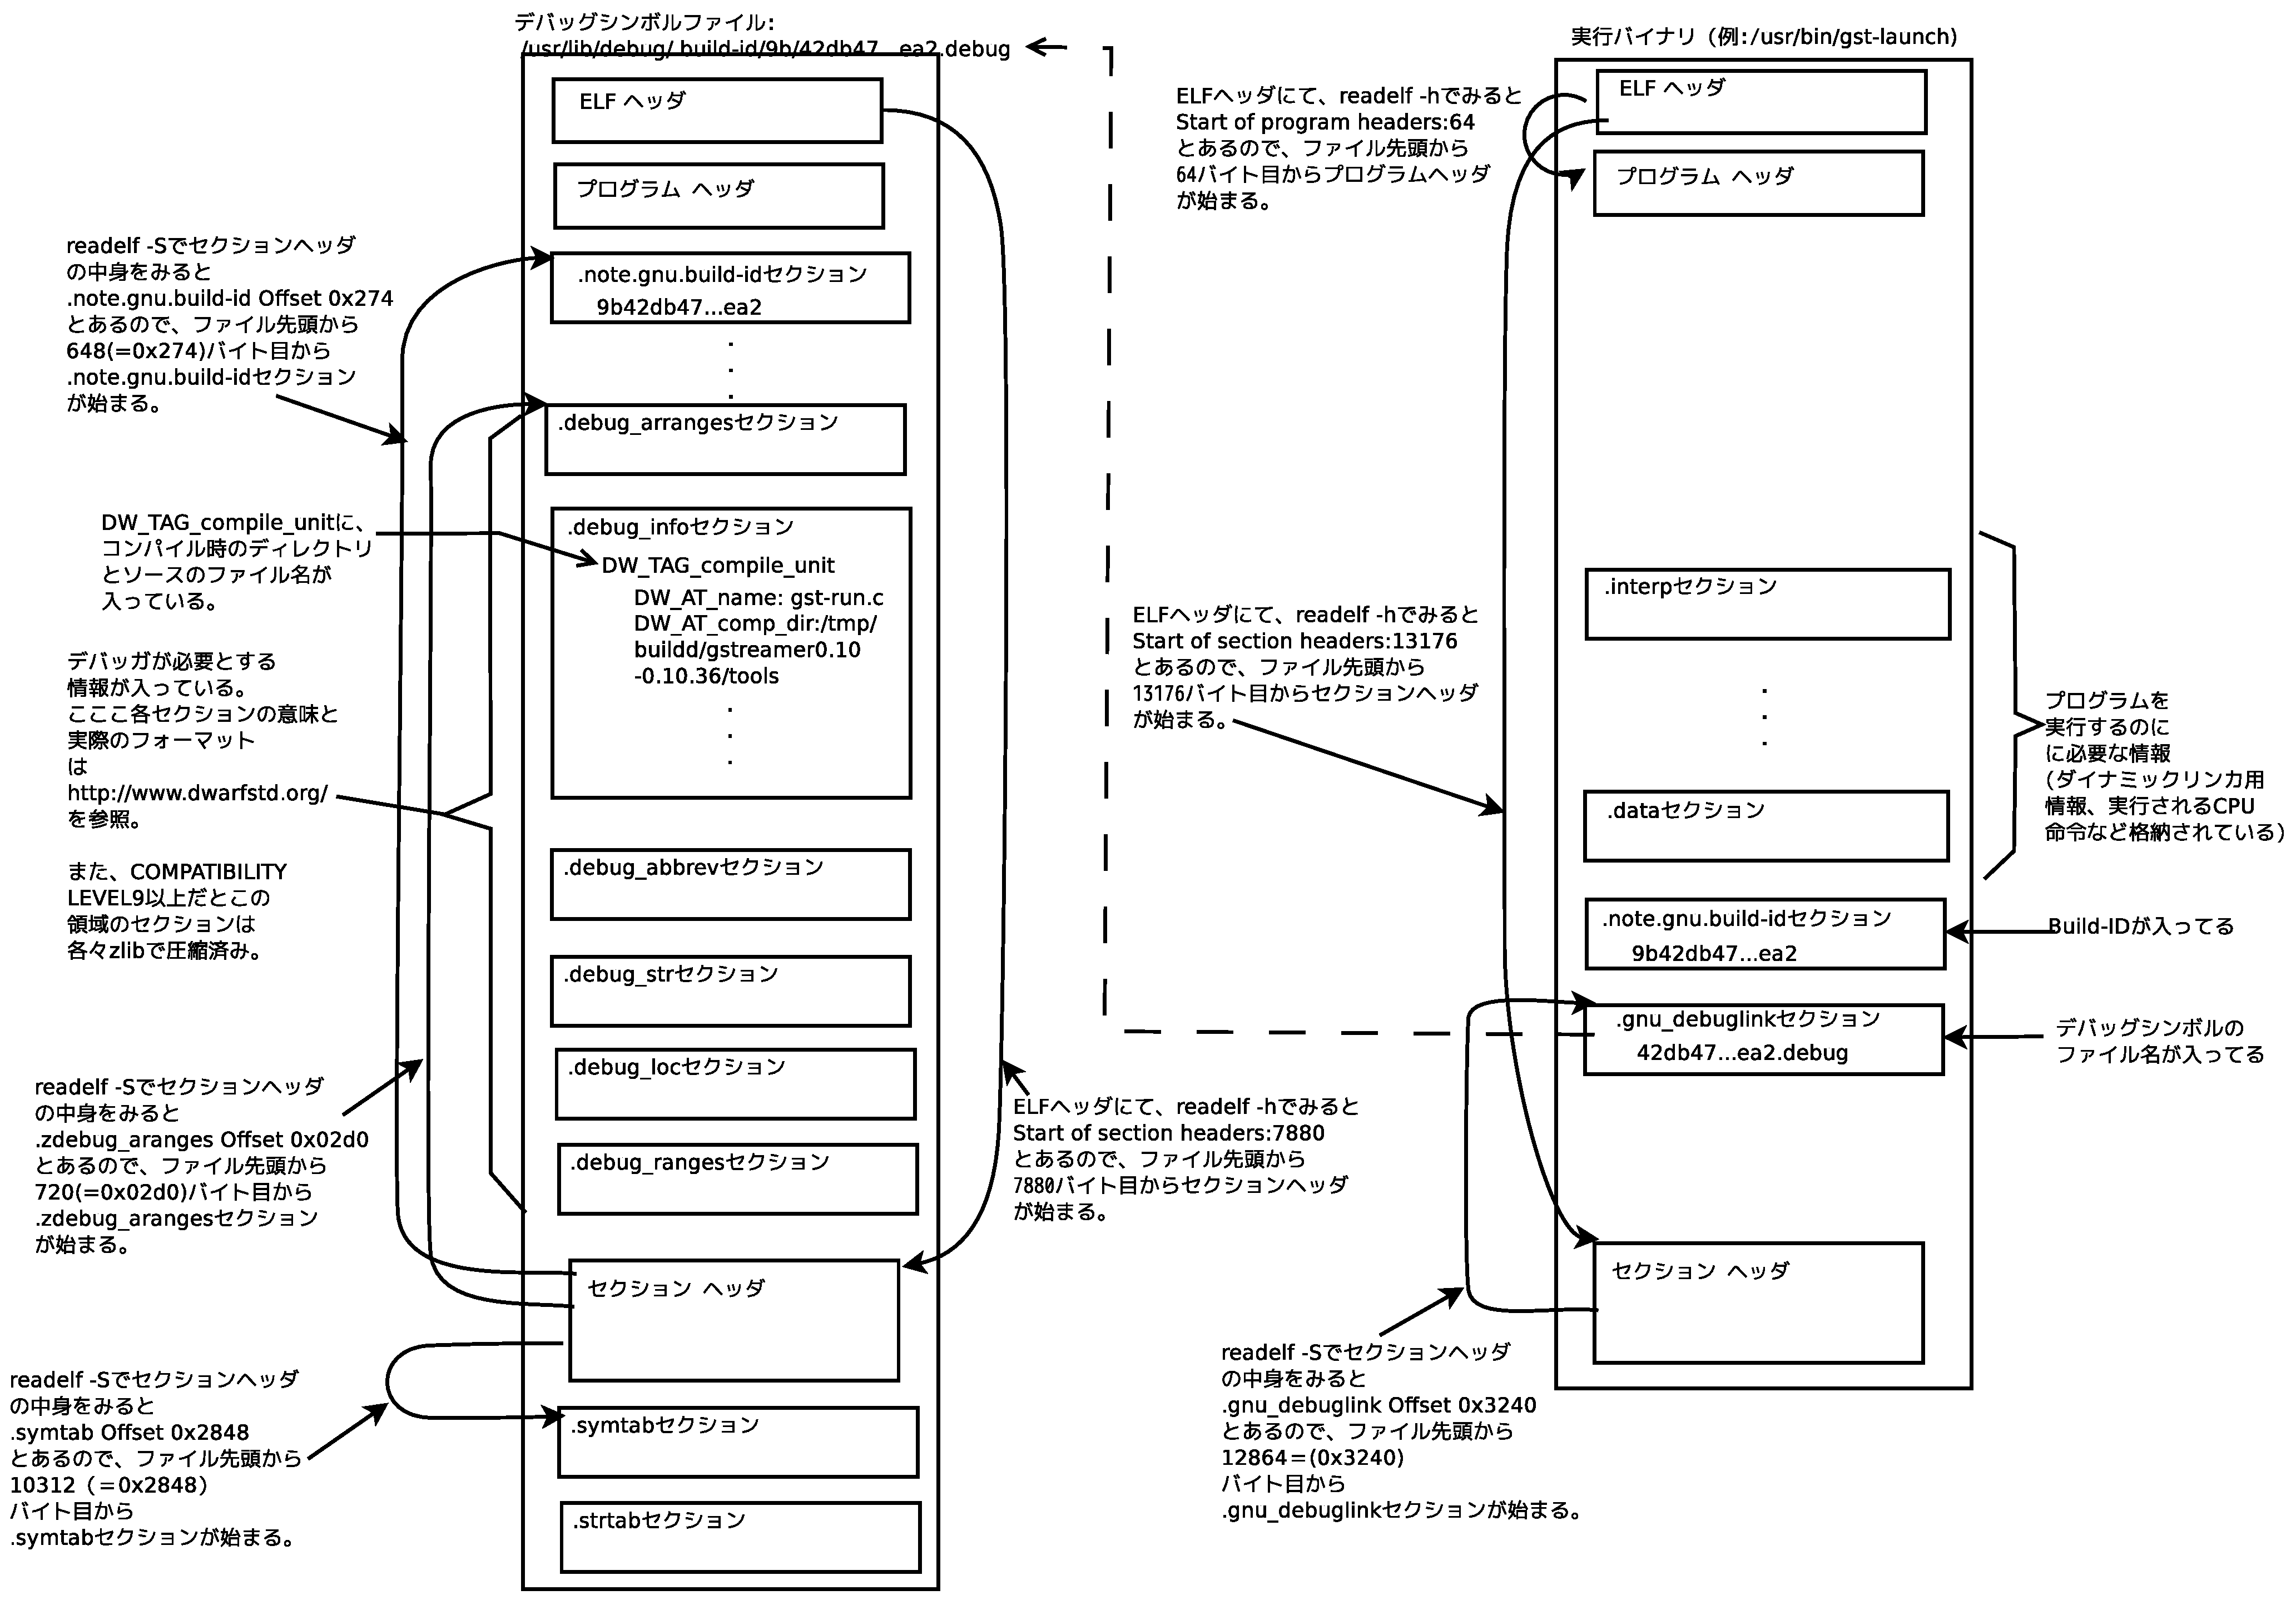
\includegraphics[width=0.8\hsize]{image201307/dwarf-elf-schema.eps}
 \caption{バイナリと、デバッグシンボルの中身}
 \label{fig:dwarf-vs-elf-schema}
\end{center}
\end{figure}

\subsubsection{デバッグシンボルファイルの情報を覗いてみる}
 
 実はバイナリや、デバッグシンボルの中身を見る方法は知っておくと、
いろいろデバッグ等で役立つ場面が多いです。以下に簡単に参照する方法を載せます。

 まず、バイナリにはどんなヘッダ情報とセクションが入っているかのサマリを
掌握してみます。

\begin{commandline}
$ sudo aptitude install binutils
$ readelf -e /usr/bin/gst-launch
ELFヘッダ
   マジック:  7f 45 4c 46 02 01 01 00 00 00 00 00 00 00 00 00 
  ...中略...
セクションヘッダ:
  [番] 名前              タイプ           アドレス          オフセット
       サイズ            EntSize          フラグ Link  情報  整列
  [ 0]                   NULL             0000000000000000  00000000
       0000000000000000  0000000000000000           0     0     0
  [ 1] .interp           PROGBITS         0000000000400238  00000238
       000000000000001c  0000000000000000   A       0     0     1
...中略...
  [27] .gnu_debuglink    PROGBITS         0000000000000000  00003240
       0000000000000034  0000000000000000           0     0     1
  [28] .shstrtab         STRTAB           0000000000000000  00003274
       00000000000000fe  0000000000000000           0     0     1
...中略...
\end{commandline}

 次にどんなデバッグシンボルファイルが使われる予定かを見てみます。

\begin{commandline}
$ readelf -x .gnu_debuglink /usr/bin/gst-launch
セクション '.gnu_debuglink' の 十六進数ダンプ:
  0x00000000 34326462 34373631 31386162 32623831 42db476118ab2b81
  0x00000010 30343161 63643830 65343565 38396534 041acd80e45e89e4
  0x00000020 32383965 61322e64 65627567 00000000 289ea2.debug....
  0x00000030 dbf8060d                            ....
$
\end{commandline}

 デバッグシンボルのファイル名の形式から、COMPATIBILITY LEVEL 9のソース
パッケージで構築されたデバッグシンボルファイルである事がわかります。
このため、BuildIDから、/usr/lib/debug/.build-id/9b/42db476118ab2b81041acd80e45e89e4289ea2.debugがデバッグシンボル
のファイルとなります。

 次にデバッグシンボルファイルから、ビルド時のディレクトリ位置を求めてみます。

\begin{commandline}
$ aptitutde install libgstreamer0.10-0-dbg
$ readelf -wi /usr/lib/debug/.build-id/9b/42db476118ab2b81041acd80e45e89e4289ea2.debug | lv
.debug_info セクションの内容:

  コンパイル単位 @ オフセット 0x0:
   長さ:        0x1b3b (32-bit)
   バージョン:    2
   Abbrev Offset: 0x0
   ポインタサイズ:8
 <0><b>: 省略番号: 1 (DW_TAG_compile_unit)
    <c>   DW_AT_producer    : (間接文字列、オフセット: 0x442): GNU C 4.7.2      

    <10>   DW_AT_language    : 1        (ANSI C)
    <11>   DW_AT_name        : (間接文字列、オフセット: 0x57a): gst-run.c       

    <15>   DW_AT_comp_dir    : (間接文字列、オフセット: 0x36b): /tmp/buildd/gstr
eamer0.10-0.10.36/tools
 ...中略...
\end{commandline}
%$

 .debug\_infoセクションに定義されている、DW\_TAG\_compile\_unitの結果から、
ディレクトリ/tmp/buildd/gstreamer0.10-0.10.36/toolsに配置されている
gst-run.cがコンパイルされている事がわかります。

 では、この結果を元に、gdbのset substitute-pathを使ってgdbでソースの
閲覧をやってみます\footnote{なお、本方法は、2013年大統一Debian勉強会\cite{gdb-python-debug2}の当時では、自分がまだ見つけていなかった方法でして...これでgdbのdirコマンドを使わなくて済み、今後は*-dbgパッケージを導入するだけで便利にソースの閲覧できるようになります。}。

\begin{commandline}
$ pwd
/home/yours/src/gstreamer/
$ apt-get source gstreamer0.10-tools/sid 
$ gdb --args /usr/bin/gst-launch
...中略...
Reading symbols from /usr/bin/gst-launch...Reading symbols from 
/usr/lib/debug/.build-id/9b/42db476118ab2b81041acd80e45e89e
4289ea2.debug...done.
(gdb) set substitute-path /tmp/buildd/ /home/yours/src/gstreamer/
(gdb) b main
(gdb) run
(gdb) l
313	  return candidates;
314	}
315	
316	int
317	main (int argc, char **argv)
318	{
319	  GHashTable *candidates;
320	  gchar *dir;
\end{commandline}
%$

無事ソース閲覧ができています。

\subsection{おわりに}

 今回は、dh\_stripコマンドをネタに、デバッグシンボルファイル
の中を覗き、その結果を元に最後はgdbでソース閲覧ができるようになる
までをやってみました。

 また、dh\_stripの周辺技術を見てみると、ソースコードのデバッグができるように
なる為に、とても多くの人の成果物を活用していることが実感できました。

\begin{thebibliography}{0}
    \bibitem{debug-debian-net}
      {\footnotesize{
          2012年大統一Debian勉強会「debug.debian.net」,
          \url{http://gum.debian.or.jp/2012/}
        }}

    \bibitem{gdb-python-debug2}
      {\footnotesize{
          2013年大統一Debian勉強会「gdb+python拡張を使ったデバッグ手法」,
          \url{http://gum.debian.or.jp/2013/slide_data_list}
        }}
    \bibitem{dwarf-spec}
      {\footnotesize{
          The DWARF Debugging Standard,
          \url{http://www.dwarfstd.org/Home.php}
        }}

\end{thebibliography}


%-------------------------------------------------------------------------------
\dancersection{raspberry pi}{上川 純一}
%-------------------------------------------------------------------------------
\index{raspberry pi}
\index{armhf}
\index{raspbian}

\subsection{はじめに}

raspberry pi は市販されている安価なARMのボードです。日本国内であればRS
Components から直販されています。

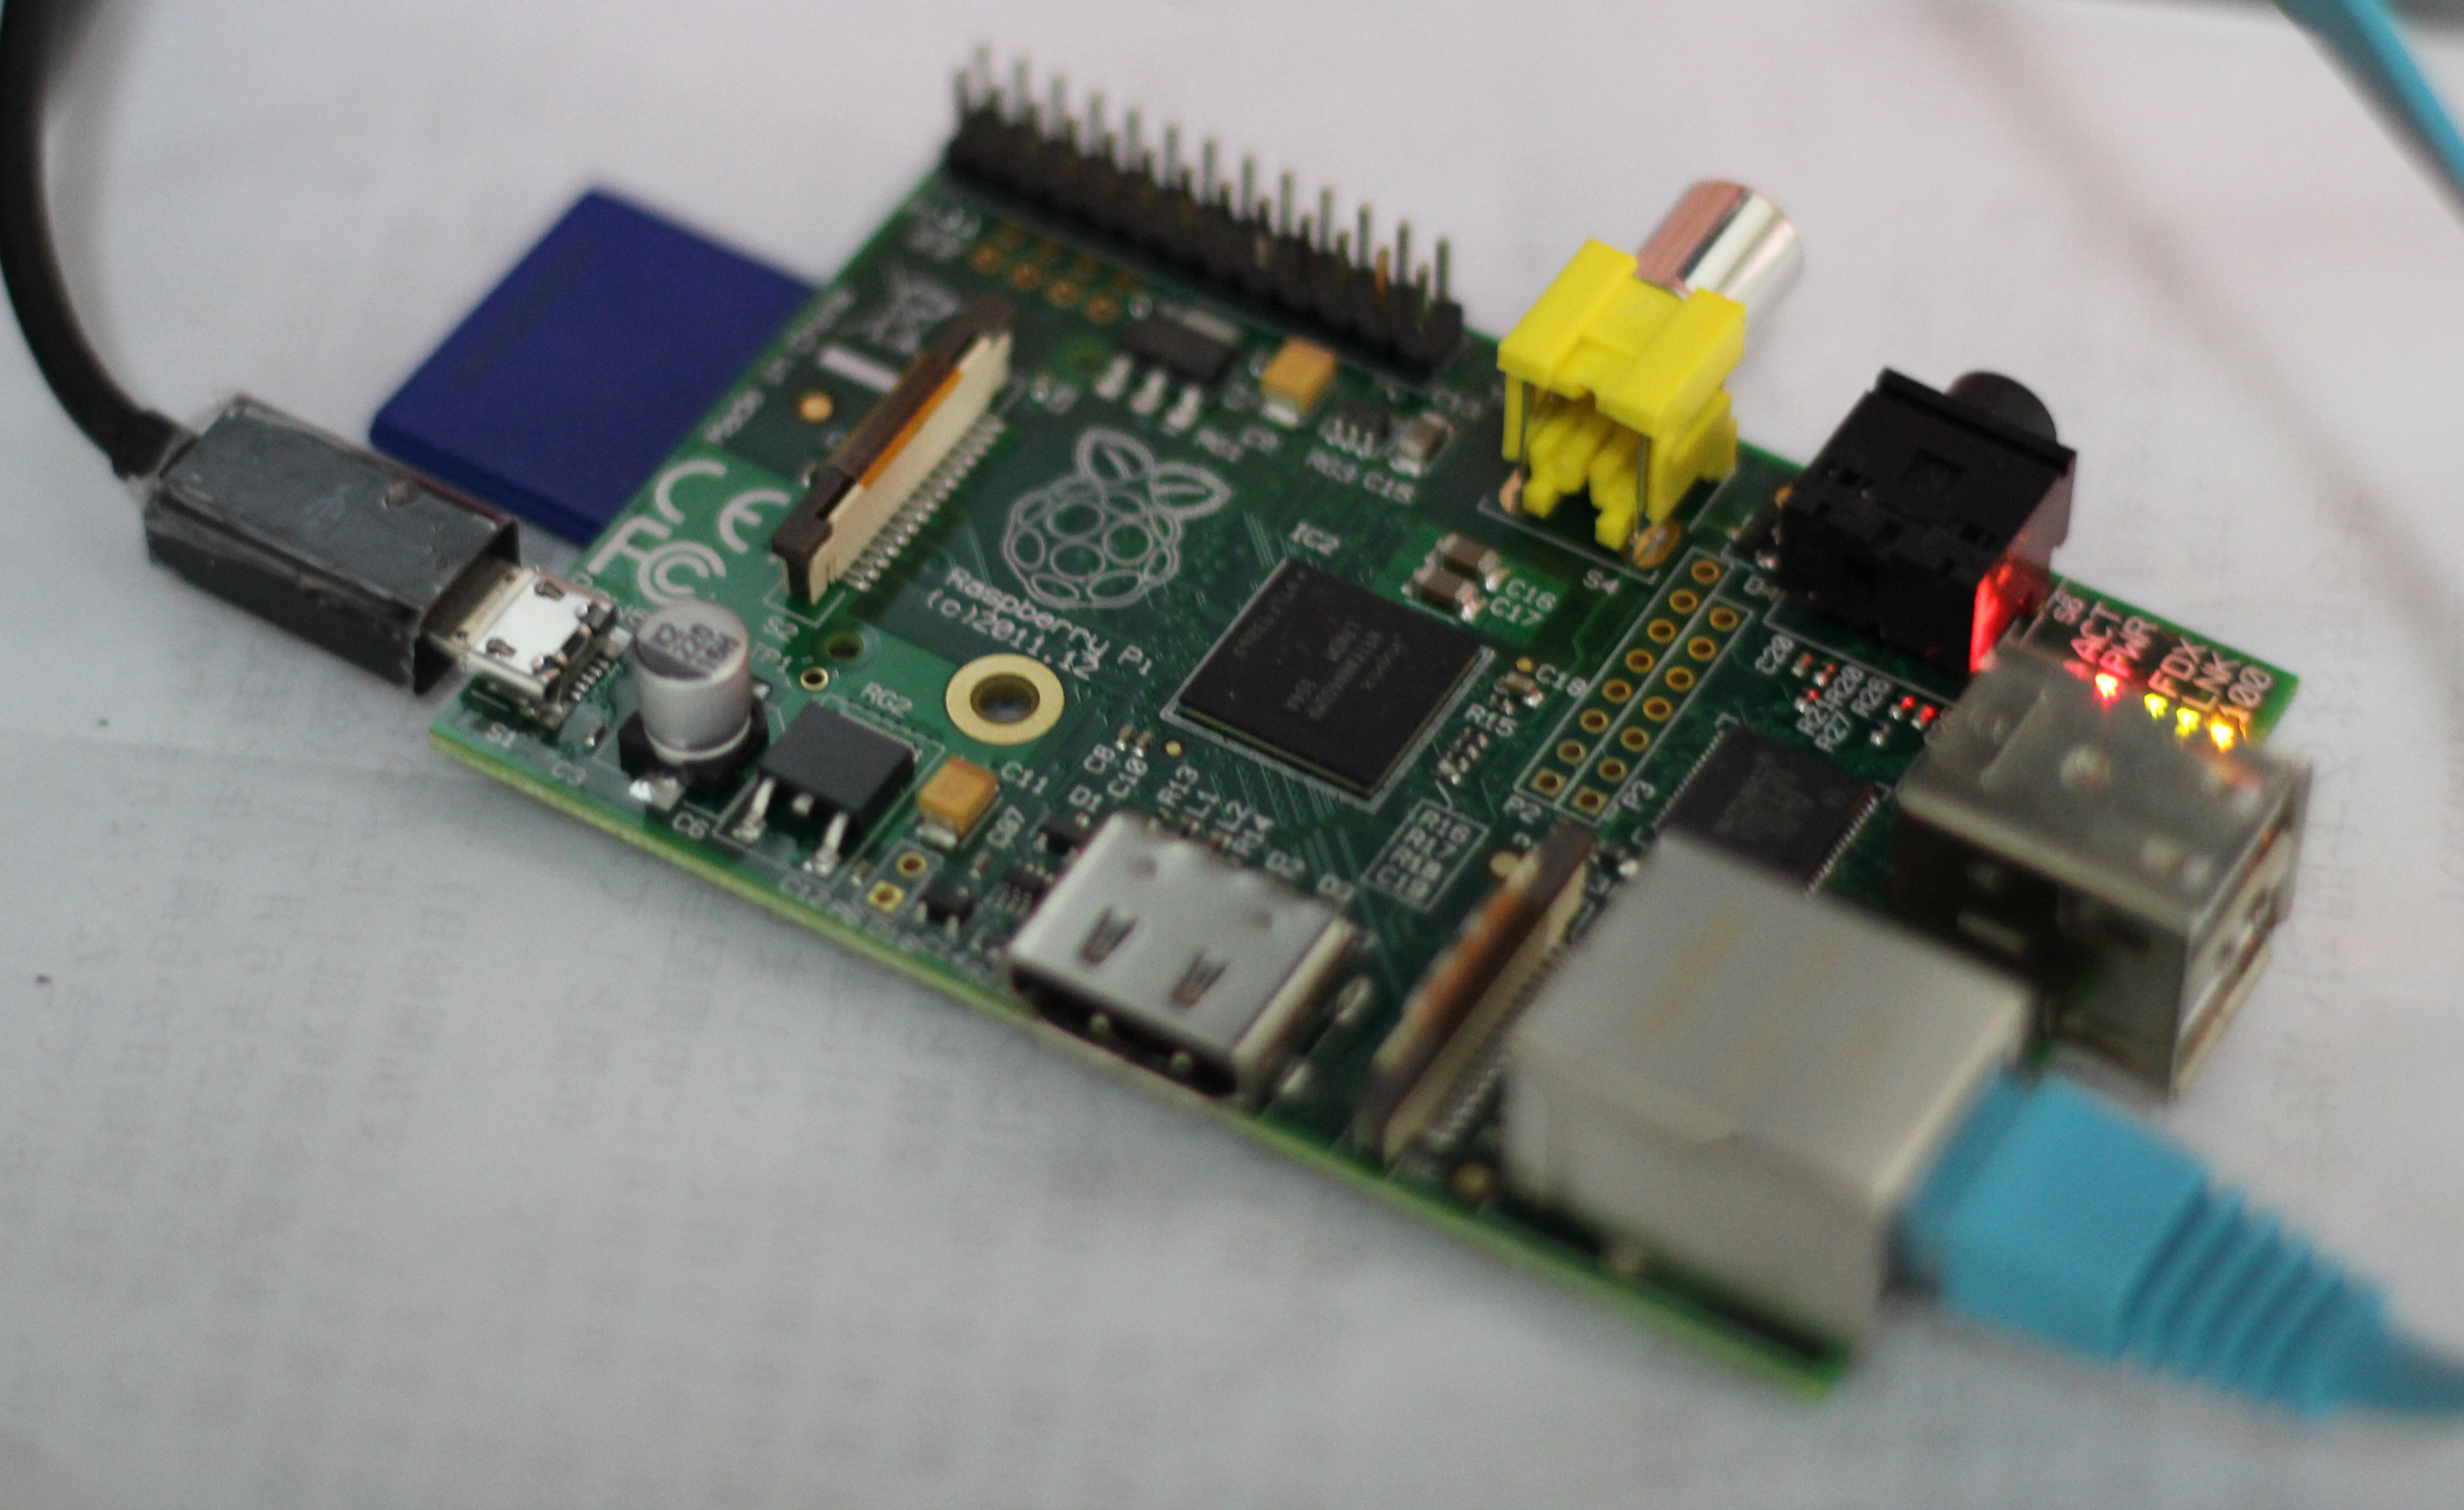
\includegraphics[width=0.5\hsize]{image201307/raspberrypi.jpg}

Debianが動くデバイスという観点でみると、CPUとして ARM1176JZF-S が搭載さ
れているデバイスです。
ARM11 (ARMv6) で、ハードウェアで浮動少数点演算ができるVFPが搭載されてお
り、ARMv7 以降の機能である NEON には対応していません。

HDMI出力、イーサネット、USBホストなどがあるため、モニタとキーボードを接続
すると普通のパソコンのように利用できるようになっています。電源はmicro
USB端子で、1A以上が供給できるようになっている最近のスマートホン用の電源で
あれば流用できます。

\subsection{Raspbian}

Raspberry pi 用のLinuxディストリビューションの一つがRaspbianです。今回は
それを採用します。

\subsubsection{Raspbianでなにがうれしいのか?}

Debian そのものではなく Raspbian を利用する理由はなんでしょうか。インストール画
面がカスタマイズされていますが、それ以外に何のメリットがあるのでしょうか。
Debian GNU/Linuxのwheezy時点の安定版でサポートされているアーキテクチャは2つあり、armelとarmhfです。

raspberry pi は armel で動作します。しかし、armel は armv4 互換で、armv6 の機能を生かしてくれません。
armv6 では VFPv2 (ARMの浮動小数点ユニット) や SIMD(整数演算がストリーミング計算できる) 命令ができ
ることになっているので、それを利用しない手はないです。
一方ハードウェア浮動小数点命令を活用する設定になっているarmhfは一方でarmv7 以上でのみ動くので、armv6 では動いてくれません。

そこで登場するのがRaspbian です。これはarmv6, VFP 対応でDebianパッケージ
をコンパイルしなおしたディストリビューションです。

アーキテクチャ名はarmhf となっており、Debianのarmhfアーキテクチャのパッケー
ジをそのままインストールすることができますが、実行してもサポートされてい
ない命令を実行した時点でエラーを出力するようです。

\begin{table}[ht]
\begin{center}
\caption{各 Debian arm アーキテクチャの違い}
  \begin{tabular}{|c|c|c|c|}
 \hline
 & dpkg アーキテクチャ表示 & 浮動小数点演算ABI & 命令セットアーキテクチャ\\
 \hline
   Debian armel & armel & soft & armv4 \\
   Debian armhf & armhf & hard & armv7 \\
   raspbian & armhf & hard & armv6 \\
 \hline
 \end{tabular}
\end{center}
\end{table}

\subsubsection{インストール}

rapbian はインストール済のSDカードを入手するという事も可能ですが、そうでない場合は
本体だけでインストールが完了する手順というのはおそらくないので、別途パソ
コンを用意してください。SDカードを用意して、配布されているSDカードの起動
イメージをddで書きこみ、本体に挿入して起動するだけでよいです。
\cite{raspberrypidownloads, raspbian}

HDMIでモニターに接続して、USBでキーボードを接続して、イーサネット\footnote{
本体には物理的にRTC(時計)が搭載されていないため、起動時に現在時刻が設定
されません。ネットワークにつながっている場合はネットワークから時間を取得
することになるので通常は問題にはならないようですが、びっくりします。
}も結線
しておきます。
電源となるUSBケーブルを接続するとLEDが点灯して起動します。
しばらく起動メッセージが表示され、完了するとメニューが表示されます。

SDカードのイメージを書き込むとなるとパーティションのサイズが気になるかも
しれませんが、ファイルシステムをSDカード全体の大きさへ拡張するなどの操作
がメニューにあります。

localeの設定とかはあとで適当にやりましょう。
\begin{commandline}
 $ sudo dpkg-reconfigure locales
\end{commandline}

\subsubsection{便利な小技}

raspberry pi 自体にHDMI出力やUSBなどがついているため、メイン開発機として
利用することも可能ではありますが、通常は別のマシンなどがあって作業するこ
とになると思います。
そのときに便利なのが avahi-daemon と sshfs です。

avahi-daemon をいれておけばmdns対応のクライアントからなら
``raspberrypi.local'' というホスト名で接続できるように
なります。

sshの設定はするだろうから、sshfs でファイルシステムをマウントしておけばファ
イルの共有が楽にできます。sshfsはsshの接続さえできればファイルシステムを
マウントできるので便利です。
個人的には最近はファイル共有は sshfs か git を使っています。
\begin{commandline}
 sshfs corei7.local:path/to/work ./mnt/
\end{commandline}

\subsubsection{Raspbian での呼び出し規約}

Raspbian(armhf)ではarmelと違い、
浮動小数点関連の関数の呼び出し規約自体も変わり、使えるレジスタとして
r0-r31だけでなくd0-d31も利用できるようになります。

具体的なコンパイル例を見てみましょう。C++ のコード例があった場合にこれが
どうコンパイルされるかを見てみます。
\begin{commandline}
  double a = 1.1;
  double b = 2.3;
  cout << a*b;
\end{commandline}

armel: mfloat-abi=soft の場合のアセンブリの出力例。
doubleがrレジスタで扱われていて、ライブラリコールが行われています。

\begin{commandline}
  30:	e50b4018 	str	r4, [fp, #-24]
  34:	e24b1014 	sub	r1, fp, #20
  38:	e8910003 	ldm	r1, {r0, r1}
  3c:	e24b301c 	sub	r3, fp, #28
  40:	e893000c 	ldm	r3, {r2, r3}
  44:	ebfffffe 	bl	0 <__aeabi_dmul>
\end{commandline}

armhf: mfloat-abi=hard のアセンブリ出力例。
ABIが変わり、dレジスタで関数呼び出しの値が渡されるようになり、vmul で掛
け算が行われています。

\begin{commandline}
  30:   e50b4018        str     r4, [fp, #-24]
  34:   ed1b6b05        vldr    d6, [fp, #-20]  ; 0xffffffec
  38:   ed1b7b07        vldr    d7, [fp, #-28]  ; 0xffffffe4
  3c:   ee267b07        vmul.f64        d7, d6, d7
  40:   e59f0028        ldr     r0, [pc, #40]   ; 70 <main+0x70>
  44:   eeb00b47        vmov.f64        d0, d7
  48:   ebfffffe        bl      0 <_ZNSolsEd>
  4c:   e3a03000        mov     r3, #0
\end{commandline}

\subsubsection{hard float はどれくらい速度向上に貢献するのか?}

気になったので掛け算の速度をベンチマークしてみたのですが、サブルーチンを
呼び出すコードになっているarmelとvmul.64 を直接呼ぶようになっているarmhf
の違いがよくわからんでした。もっと劇的に違うと思ったのに。

\begin{commandline}
double mulbench(int iter, double a, double b) {
  double c;
  for (int i = 0; i < iter; ++i) {
    c = a * b;
  }
  return c;
}

int main(int argc, char** argv) {
  cout << mulbench(atoi(argv[1]), 1.2, 3.5) << endl;
  return 0;
}
\end{commandline}

\begin{table}
 \caption{1000000000 回 double の掛け算を行うループを実行するのにかかる時
 間(秒)、一回試行}
\begin{center}
 \begin{tabular}{|c|c|c|c|}
 \hline
 & armel & armhf & amd64(corei7) \\
 \hline
 -O1 & 4.5 & 4.6 &  0.35 \\
 -O0 & 134 & 130 &  2.6 \\
 \hline
 \end{tabular}
\end{center}
\end{table}

\subsection{raspberry pi にデフォルトで搭載されているセンサー}

Raspberry pi は外部センサーを付けないと何もできない感じがしますが実は一
部計測できるものもあります。
電圧とCPUの温度がそれです。

温度を表示してみましょう。ミリ度C で表示されるようです。今の温度は55度の
ようです。
\begin{commandline}
$ cat /sys/class/thermal/thermal_zone0/temp
 55148
\end{commandline}

時系列で温度のグラフを作ってみました。

\begin{figure}[H]
 \begin{center}
  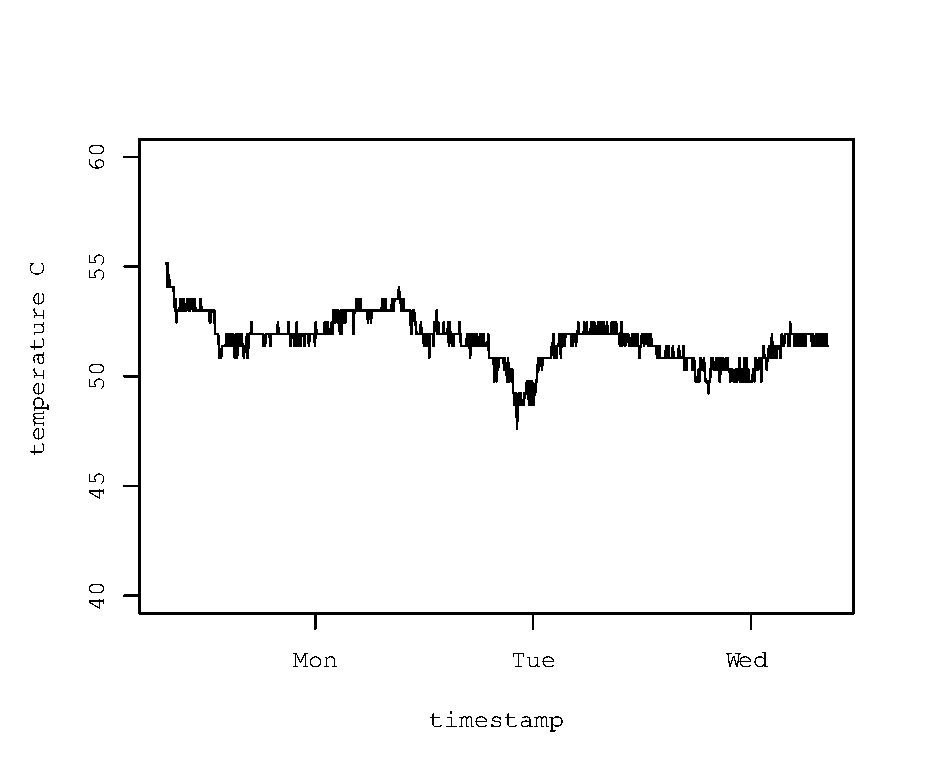
\includegraphics[width=0.5\hsize]{image201307/temperature.eps}
  \caption{Raspberry pi CPU 温度(℃)の時系列での変化}
 \end{center}
\end{figure}

この温度センサーの値は0.001℃単位(m℃?)で取得できますが、結果を見た限り
では実際に取得できる値は連続ではなく離散的で、538 m℃ 単位のようです。

\subsection{おわりに}

Raspberry Piを購入してみて二ヶ月くらい放置していたのですが、いいかげんた
ちあげて見ました。しかしまだ長期的に何をさせるのかは考え中。

\begin{thebibliography}{}
 \bibitem{raspberrypidownloads} raspberry pi のソフトウェアダウンロードサイト (raspbianへのリンクが貼っ
てある)
\url{http://www.raspberrypi.org/downloads}
 
\bibitem{raspbian} raspbian のサイト \url{http://www.raspbian.org/}
\end{thebibliography}


\printindex

\cleartooddpage

\vspace*{15cm}
\hrule
\vspace{2mm}

\includegraphics[width=2cm]{image200502/openlogo-nd.eps}
\noindent \Large \bf Debian 勉強会資料\\
\noindent \normalfont \debmtgyear{}年\debmtgmonth{}月\debmtgdate{}日 \hspace{5mm}  初版第1刷発行\\
\noindent \normalfont 東京エリア Debian 勉強会 (編集・印刷・発行)\\
\hrule

\end{document}
